\section{Főfeszültségek}

\subsection{Mohr-féle diagram}

\begin{align*}
	\tau_{xy} = \tau_{yz} = 0 &\Rightarrow \sigma_y = 0 \\
				  &\Rightarrow \pmb{e_2} = \begin{bmatrix}
		0 \\
		1 \\
		0
	\end{bmatrix} \\ 
				  &\Rightarrow \sigma_2 = 0
\end{align*}

\begin{align*}
	&X(\sigma_x; \left[\tau_{xz}\right]) = (-99.231; 54.9231) \\
    	&Y(\sigma_y; 0) = (0; 0) \\
	&Z(\sigma_z; \left[\tau_{xz}\right]) = (33.231; 54.9231) \\
\end{align*}

\begin{align*}
	\sigma_\text{K} &= \frac{\sigma_x + \sigma_z}{2} = \mpa{-33} \\
	R &= \sqrt{\left(\frac{\sigma_x - \sigma_z}{2}\right)^2 + \tau_{xz}^2} = \mpa{86.04122}
\end{align*}

\begin{align*}
	\sigma_{1;3} = \sigma_\text{K} \pm R = \begin{cases}
		53.04122 \\
		-119.04122
	\end{cases}
\end{align*}

\begin{center}
	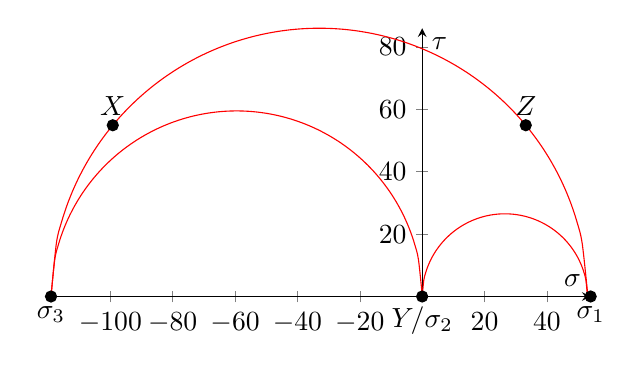
\begin{tikzpicture}
		\begin{axis}[
			axis lines=middle,
			clip=false,
			axis equal image,
			xlabel = {$\sigma \mpa{}$},
			ylabel = {$\tau \mpa{}$},
		]
		\addplot[only marks, mark=*] coordinates {(-99.231, 54.9231)} node [above] {$X$};
		\addplot[only marks, mark=*] coordinates {(0,0)} node [below] {$Y / \sigma_2$};
		\addplot[only marks, mark=*] coordinates {(33.231, 54.9231)} node [above] {$Z$};

		\addplot[only marks, mark=*] coordinates {(-119.04122, 0)} node [below] {$\sigma_3$};
		\addplot[only marks, mark=*] coordinates {(54.04122, 0)} node [below] {$\sigma_1$};

		\addplot[domain=-119.04122:53.04122, samples=100, smooth, red] {sqrt((86.04122)^2-(x + 33)^2)};
		\addplot[domain=-119.04122:0, samples=100, smooth, red] {sqrt((59.52061)^2-(x + 59.52061)^2)};
		\addplot[domain=0:53.04122, samples=100, smooth, red] {sqrt((26.52061)^2-(x - 26.52061)^2)};
		\end{axis}
	\end{tikzpicture}
\end{center}

\subsection{Főirányok}
\begin{align*}
	\phi_1 &= \text{arctg}(\frac{\sigma_1 - \sigma_x}{\tau_{xz}}) = \ang{70.166} \\
	\pmb{e_1} &= \begin{bmatrix}
		\cos \phi_1 \\
		0 \\
		-\sin \phi_1
		\end{bmatrix} = \begin{bmatrix}
			0.3393 \\
			0 \\
			-0.941
		\end{bmatrix} \\
	\pmb{e_3} &= \pmb{e_1} \times \pmb{e_2} = \begin{bmatrix}
		0.941 \\
		0 \\
		0.3393
	\end{bmatrix}
\end{align*}

\newpage

\subsection{Ellenőrzés}

\subsubsection{Sajátérték}
\begin{align*}
	\text{det}(\pmb{\sigma} - \lambda\pmb{E}) &= 0 \\
	\begin{bmatrix}
		\sigma_x - \lambda & 0 & 0 \\
		0 & -\lambda & 0 \\
		\tau_{xz} & 0 & \lambda_z - \lambda
	\end{bmatrix} &= 0 \\
	(-\lambda)\left[(\sigma_x - \lambda)(\sigma_z - \lambda) - \tau_{xz}^2\right] &= 0 \\ \\
	\lambda_{1;2;3} &= \begin{cases}
		53.04122 \\
		0 \\
		-119.04122
	\end{cases} \\&= \sigma_{1;2;3} \; \checkmark
\end{align*}

\subsubsection{Sajátvektor}
A főírányok merőlegessége miatt írható fel a következő egyenlet.
\begin{align*}
	\pmb{\sigma} - \lambda_1 \pmb{E} &= \pmb{0} \\
	\begin{bmatrix}
		\sigma_x - \sigma_1 & 0 & \tau_{xz} \\
		0 & 0 & 0 \\
		\tau_{xz} & 0 & \sigma_z - \sigma_1 
	\end{bmatrix} \begin{bmatrix}
		\cos \phi \\
		0 \\
		\sin \phi
	\end{bmatrix} &= \pmb{0} \\
\end{align*}

\begin{align*}
	(\sigma_x - \sigma_1)\cos \alpha + \tau_{xz} \sin \alpha &= 0 \\
	 \tau_{xz} \cos \alpha + (\sigma_z - \sigma_1)\sin \alpha &= 0 \\
\end{align*}

\begin{align*}
	 \frac{\cos \alpha}{\sin \alpha} &= -\frac{\sigma_z - \sigma_1 + \tau_{xz}}{\sigma_x - \sigma_1 + \tau_{xz}} \\
	 \alpha &= \ang{70.1661} = \phi \checkmark
\end{align*}

